\subsection{Conceptos}
\begin{itemize}
    \item \textbf{Interrupciones:} Consiste en una notificación al CPU que un evento ha sucedido. Es decir, tiene prioridad sobre el programa y ocurre en paralelo y no de una forma secuencial o siguiendo un control de flujo. Es decir, si se está dentro de un \texttt{while} por ejemplo, y ocurre el evento de interés, entonces se interrumpe el procesamiento general para atender la interrupción. Pueden ser disparadas por varios eventos/periféricos como I/Os, ADC, software, timers, entre otros. \cite{presentacion}. Las rutinas de interrupción (o la lógica que está dentro de la interrupción) debe ser \textbf{muy corta}. Funciona bajo el siguiente flujo: Ocurre evento -> Se dispara interrupción y el programa se detiene -> Se guarda el estado actual del programa -> El procesador revisa el espacio de memoria de registro de interrupciones (Vectores de interrupción) -> Se ejecuta la subrutina de interrupción -> EL programa continúa. La imagen a continuación indica la prioridad en la que se ejecutan las interrupciones \cite{presentacion}. 
\begin{figure}[H]
\centering
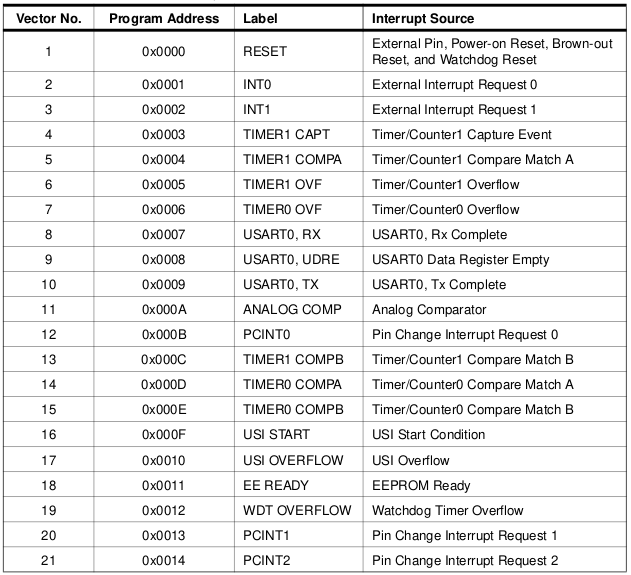
\includegraphics[scale=0.9]{./images/vector.png} 
\caption{Vector de interrupciones \cite{datasheet}.}
\label{f1}
\end{figure}

\item \textbf{Timers:} Son periféricos que permiten medir intervalos de tiempo y pueden generar interrupciones. La velocidad con la que estos perifericos cuentan está en función de la velocidad de reloj del MCU y la configurración del \textit{prescaler}. El generador de relojes del MCU opera a una frecuencia muy alta para la percepción humana. Entonces a través del prescaler se puede configurar una frecuencia de reloj más lenta. El prescaler es un circuito contador/divisor que permite entonces reducir una señal eléctrica de ala frecuencia por medio de fracciones. Existen diferentes prescalers para diferentes periféricos del circuito \cite{presentacion}.
    
\end{itemize}